\section{Introduction}

% defining? fundamental?
A quintessential characteristic of computational artificial life experiments is the near total malleability of the simulacrum \citep{pattee1989simulations}.
Indeed, exploration of arbitrary possibilities `as they could be' is the core of artificial life's role as a tool for inquiry \citep{langton1997artificial}.
Such near-limitless freedom to realize arbitrary system configurations, however, can obscure an intrinsic limitation of most computational artificial life work: scale.

Take, for instance, the Avida platform, which instantiates populations of self-replicating computer programs for evolution experiments.
When running on a single CPU, this system can support about 20,000 generations per day, or about two hundred million individual replication cycles daily \citep{ofria2009artificial}.
By way of comparison, \textit{E. coli} populations within individual flasks of the Lenski Long-Term Evolution Experiment undergo only six doublings per day, meaning their generations take orders of magnitude longer than Avidians \citep{good2017dynamics}.
(In continuous culture, though, the rate can be c. 72 generations per day.)
Indeed, such capability for fast generational turnover has been a key motivation for using artificial life systems to study evolution.
However, the effective population size of flasks in the Long-Term Evolution Experiment is orders of magnitude larger than Avida's: 30 million vs. 10,000.
Consequently, these systems actually exhibit a similar number of replication events per day.
This pattern of dramatically faster generation times than those observed in nature and dramatically smaller populations largely generalizes across artificial life systems.
%Although alife systems can typically observe generational cycles at orders-of-magnitude faster rates than their biological counterparts, population sizes are often limited and,
Of course, any such comparisons should also note profound discrepancies between the genetic, phenotypic, and environmental richness of biological organisms and alife models.

% Adversely? Crucially? Conversely? Formidably? Aversely? Cumbrously?
Crucially, however, the scale of population size can greatly impact subjects of artificial life research, like transitions in individuality, ecological dynamics, and rare evolutionary innovations \citep{taylor2016open,dolson2021digital,taylor2019evolutionary}.
Cross-scale dynamics are also crucial to many key real-world challenges.
For example, in evolutionary epidemiology, interactions between within-host infection dynamics and population-level epidemiological patterns determine the evolutionary trajectory of the population \citep{schreiber2021cross}.
However, because capabilities of current silicon-based processors are not expected to improve markedly in the foreseeable future \citep{sutter2005free}, scale-up necessary to progress on these key frontiers will demand many-processor computation.
Application of parallel and distributed computation, however, imposes compromises to the convenience, flexibility, observability, interpretability, total reliability, and perfect replicability enjoyed under classical centralized, serial models of computation.
Encouragingly, these challenges are already implicit to much of biology; the productivity of research involving natural organisms evidences that they are surmountable and even hints at strategies that can be used to solve them.
Here, we explore alignment of digital evolution to HPC accelerator hardware at the extreme cutting edge of massively distributed computation, and use techniques inspired by those applied to natural organisms to mitigate limitations of distributed computation with respect to tracking phylogenies.

\subsection{Progress Toward Scale-up in Artificial Life}

Achieving highly scalable artificial life and digital evolution systems involves two distinct engineering considerations.
First, as with any high-performance scientific computing, careful design is required to appropriately divvy computation and communication workloads across available hardware.
Second, given the exceptionally discretionary nature of artificial life modeling, we can intentionally tailor simulation semantics to suit underlying hardware capabilities.
Ackley's ongoing work with the T2 Tile Project and ULAM exemplifies a strong synthesis of this engineering duality \citep{ackley2016ulam}.
At the level of simulation semantics, Ackley formulates update procedures in terms of local interactions between discrete, spatially situated particles.
This design provides for efficient one-to-one mapping between simulation space and hardware components, minimizing requirements for intra-hardware connectivity and preventing global impacts from on-the-fly augmentations or reductions of available hardware.
The ULAM framework then ties into implementation-level infrastructure necessary to accomplish performant, best-effort lock/release of spatial event windows spanning bordering hardware units \citep{ackley2013movable}.
% The Santa Fe Board project provided analogous infrastructure foundations for earlier work, coordinating efficient packet-framed, non-blocking communication between hardware tile elements \citep{livingcomputationSFBSanta}.
Ackley's work is distinguished, in fact, in dipping to a yet-lower level of abstraction and tackling design of bespoke, modular distributed processing hardware \citep{ackley2011homeostatic,ackley2023robust,livingcomputationSFBSanta}.

Several additional digital evolution projects have made notable headway in synthesizing artificial life models with sophisticated, scalable technical backing, achieving rich interactions among numerous parallelized simulation components.
Harding demonstrated large-scale cellular automata-based artificial development systems, achieved through GPU-parallelized instantiations of a genetic program  \citep{harding2007fast_ieee}.
Early work by Ray with Network Tierra used an island model to distribute digital organisms across federated servers, with migration handled according to the real-time latencies and topology of the underlying network \citep{ray1995proposal}.
More recently, Heinemann's continuation of the ALIEN project has leveraged GPU acceleration to achieve spectacularly elaborate simulations with rich interactions between numerous spatially-situated soft body agents \citep{heinemann2008artificial}.
Likewise, the Distributed Hierarchical Transitions in Individuality (DISHTINY) project has incorporated event-driven agent-agent interaction schemes amenable to best-effort, asynchronous interlocution \citep{moreno2022exploring,moreno2021conduit}.
GPU-first agent-based modeling (ABM) packages like Flame GPU also tackle this problem of hardware-simulacrum matching, albeit framed at a higher level of abstraction \citep{richmond2010high}.
Beyond alife, broader realms of application-oriented evolutionary computation have folded in with many-processor computation, most commonly through island-model and director-worker evaluation paradigms \citep{abdelhafez2019performance,cantu2001master}.

\subsection{Untapped Emerging Hardware}

In retrospect, connectionist artificial intelligence turns out to have been profoundly scale-dependent.
The utility and ubiquity of ANNs have exploded in tandem with torrential growth in training set sizes, parameter counts, and training FLOPs \citep{marcus2018deep}.
Recruitment of multi-GPU training for image classification, requisite particular accommodating adjustments to the underlying deep learning architecture, is commonly identified as the watershed moment to this transformation
 \citep{krizhevsky2012imagenet}.
Commercial investment in AI capabilities then set in motion a virtuous cycle of further-enabling hardware advances \citep{jouppi2017datacenter}.
Indeed, the scaling relationship between deep learning and training resources has itself become a major area of active study, with expectation for this virtuous cycle to continue through the foreseeable future \citep{kaplan2020scaling}.

A major upshot of the deep learning race is the emergence of spectacularly capable next-generation compute accelerators \citep{zhang2016cambricon,emani2021accelerating,jia2019dissecting,medina2020habana}.
Although tailored expressly to deep learning workloads, these hardware platforms represent an exceptional opportunity to leapfrog progress on grand challenges in artificial life.
The emerging class of fabric-based accelerators, led by the 850,000 core Cerebras CS-2 Wafer Scale Engine (WSE) \citep{lauterbach2021path,lie2022cerebras}, holds particular promise as a vehicle for artificial life models.
This architecture interfaces multitudinous processing elements (PEs) in a physical lattice, with PEs executing independently with private on-chip memory and interacting locally through a network-like interface.

Our work here explores how such hardware might be recruited for large-scale digital evolution, demonstrating a genetic algorithm implementation tailored to the dataflow-oriented computing model of the CS-2 platform.
Indeed, rapid advances in the capability of accelerator devices, driven in particular by market demand for deep learning operations, are anticipated to drive advances in agent-based model capabilities \citep{perumalla2022computer}.
The upcoming CS-3 chip, for instance, supports clustering potentially thousands of constituent accelerators \citep{moore2024cerebras}.


\subsection{Maintaining Observability}

Orthogonalities between the fundamental structure and objectives of AI and artificial life methods will complicate any effort to requisition AI hardware for artificial life purposes.
In common use, deep learning operates as a black box medium \citep{loyola2019black} (but not always \citep{mahendran2015understanding}).
This paradigm de-emphasizes accessibility of inner state.
In contrast, artificial life more often functions as a tool for inquiry.
This goal emphasizes capability to observe and interpret underlying simulation state \citep{moreno2023toward,horgan1995complexity}.
(A similar argument holds for alife work driven by artistic objectives, as well.)

Unfortunately, scale complicates simulation observability.
It is not uncommon for the volume and velocity of data streams from contemporary simulation to outstrip hardware bandwidth and storage capacity \citep{osti_1770192}.
Intentional engineering effort will be required to ensure large-scale simulation retains utility in pursuing rigorous hypothesis-driven objectives.

Here, we confront just a single aspect of simulation observability within distributed evolutionary simulation: phylogenetic history (i.e., evolutionary ancestry relationships).
Phylogenetic history plays a critical role in many evolution studies, across study domains and \textit{in vivo} and \textit{in silico} model systems alike \citep{faithConservationEvaluationPhylogenetic1992,STAMATAKIS2005phylogenetics,frenchHostPhylogenyShapes2023,kim2006discovery,lewinsohnStatedependentEvolutionaryModels2023a,lenski2003evolutionary,moreno2021case}.
Phylogenetic analysis can trace the history of notable evolutionary events (e.g., extinctions, evolutionary innovations), but also characterize more general questions about the underlying mode and tempo of evolution \citep{moreno2023toward,hernandez2022can,shahbandegan2022untangling,lewinsohnStatedependentEvolutionaryModels2023a}.
Particularly notable, recent work has used comparison of observed phylogenies against those produced under differing simulation conditions to test hypotheses describing underlying dynamics within real-life evo-epidemiological systems \citep{giardina2017inference,voznica2022deep}.
Additionally, \textit{in silico}, phylogenetic information can even serve as a mechanism to guide evolution in application-oriented domains \citep{lalejini2024phylogeny,lalejini2024runtime,murphy2008simple,burke2003increased}.

\subsection{Decentralized Phylogenetic Tracking}

\begin{figure*}
  \centering
  \begin{subfigure}[t]{0.43\linewidth}
    \centering
  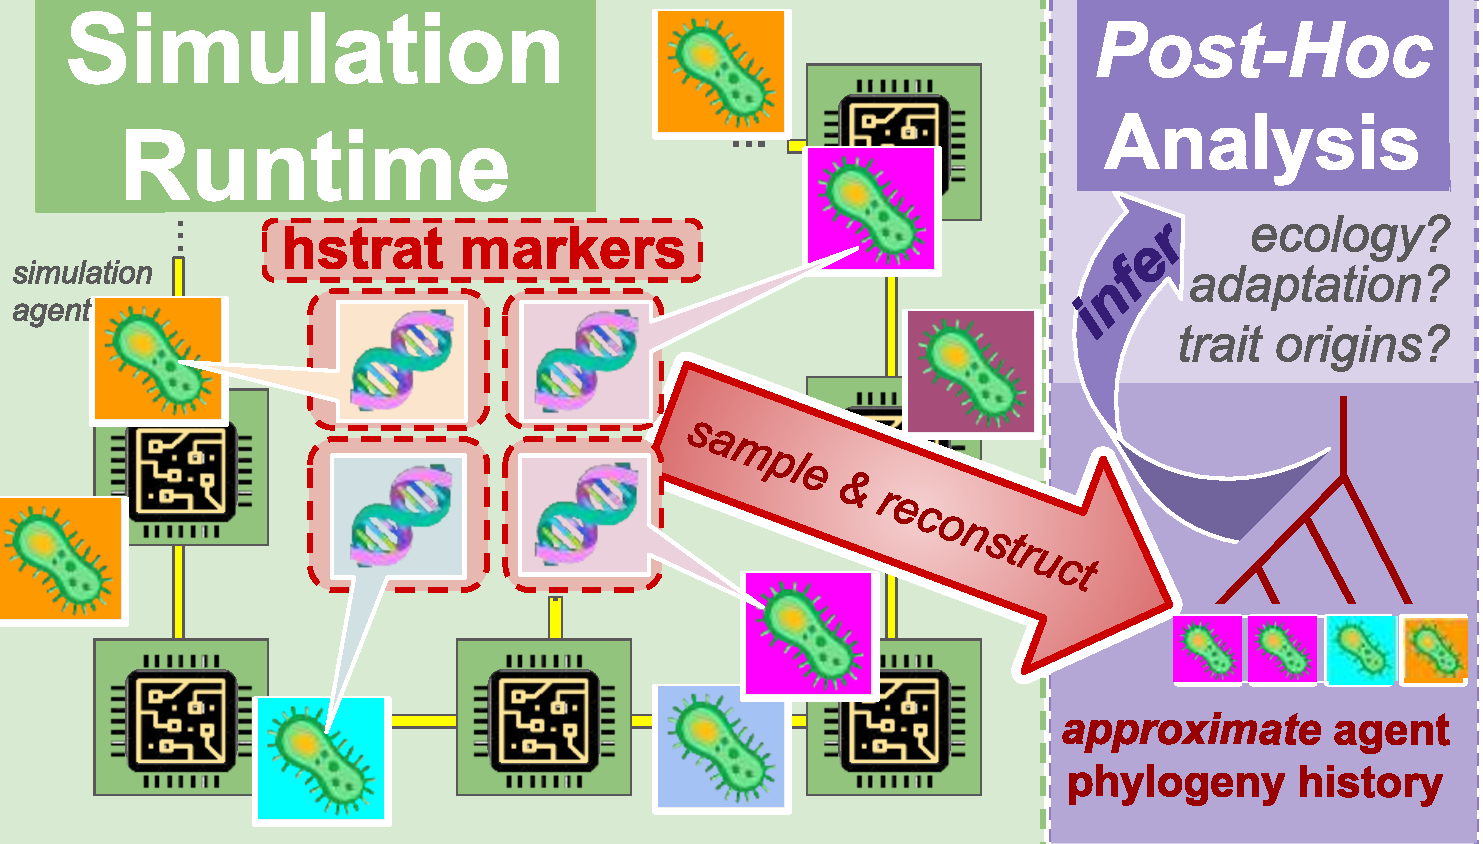
\includegraphics[width=\linewidth]{binder-wse-sketches/tex-access-proposal/img/runtime-posthoc-schematic}
    \caption{\footnotesize %
    hstrat markers help reconstruct phylogenies, which can tell evolutionary dynamics.
    }
    \label{fig:runtime-posthoc-schematic}
  \end{subfigure}
  \hspace{0.07\linewidth}
  \begin{subfigure}[t]{0.43\linewidth}
    \centering
  \includegraphics[width=\linewidth]{binder-wse-sketches/tex-access-proposal/img/async-ga-schematic}
    \caption{\footnotesize WSE island model evolutionary algorithm implementation.}
    \label{fig:async-ga-schematic}
  \end{subfigure}

\caption{%
\textbf{Methods for trackable distributed evolution simulation.}
\footnotesize
Subfigure \ref{fig:runtime-posthoc-schematic} shows use of hstrat markers to for reconstruct-based phylogenetic tracking of highly-distributed evolution simulations.
Subfigure \ref{fig:async-ga-schematic} summarizes asynchronous, callback-based approach to population exchange (``migration''') used to instantiate evolving populations across WSE PEs.
}
\label{fig:schematic}

\end{figure*}


Most existing artificial life work uses centralized tracking to maintain an exact, complete record of phylogenetic history comprising all parent-offspring relationships that have existed over the course of a simulation \citep{ray1992evolution,bohm2017mabe,de2012deap,garwood2019revosim,godin2019apoget,dolson2024phylotrackpy}.
Typically, records of extinct lineages are pruned to prevent memory bloat \citep{moreno2024analysis}.
Although direct-tracking is well suited to serial simulation or centralized controller-worker schemes, runtime communication overheads and sensitivity to data loss impede scaling to highly distributed systems --- particularly those with lean memory capacity like the Cerebras WSE \citep{moreno2024analysis}.
To overcome this limitation, we have developed reconstruction-based approaches to \textit{in silico} phylogenetic tracking \citep{moreno2022hereditary}.
These approaches require no centralized data collection during simulation runtime; instead, they use \textit{post hoc} comparisons among end-state agent genomes to deduce approximate phylogenetic history --- akin to how DNA-based analyses describe natural history.
Figure \ref{fig:runtime-posthoc-schematic} summarizes this reconstruction-based strategy.

Although analogous work with natural biosequences is notoriously challenging and data-intensive \citep{neyman1971molecular,lemmon2013high},
the recently-developed hereditary stratigraphy annotation architecture is explicitly designed for fast, accurate, and data-lean reconstruction.
% Work reported here uses just 96 bits of tracking information per agent genome.
Designed to attach on underlying replicators as a neutral annotation (akin to noncoding DNA), it is a general-purpose technique potentially applicable across diverse study domains \citep{liben2008tracing,cohen1987computer,friggeri2014rumor}.
In a stroke of convergent thinking, \citet{ackley2023robust} reports use of ``bar code'' annotations on his self-replicators to achieve a measure of coarse-grained lineage tracing.

\subsection{Contributions}

In this paper, we report new software and algorithms that harness the Cerebras Wafer Scale Engine to enable radically scaled-up agent-based evolution while retaining key aspects of observability necessary to support hypothesis-driven computational experiments.
Implementation comprises two primary aspects:
\begin{enumerate}
  \item an asynchronous island-based genetic algorithm (GA) suited to the memory-scarce, highly-distributed, data-oriented WSE architecture, and
  \item a fundamental reformulation of hereditary stratigraphy's core storage and update procedures to achieve fast, simple, resource-lean annotations compatible with unconventional, resource-constrained accelerator and embedded hardware like the WSE.
\end{enumerate}

Both are implemented in Cerebras Software Language (CSL) and validated using Cerebras' SDK hardware emulator.
We use benchmark experiments to evaluate the runtime performance characteristics of the new hereditary stratigraphy algorithms in isolation and in the integrated context providing tracking-enabled support for the island-model GA.
In conjunction, we report emulated and on-device trials that validate phylogenetic reconstructions and demonstrate their suitability for inference of underlying evolutionary conditions.

Results from both experiments are promising.
We find that new surface-based algorithms greatly improve runtime performance.
Scaled-down emulator benchmarks and early on-hardware trials indicate potential for simple agent models --- with phylogenetic tracking enabled --- to achieve on the order of quadrillions of agent replication events a day at full wafer scale, with support for population sizes potentially reaching hundreds of millions.
Further, using proposed techniques, phylogenetic analyses of simulations spanning hundreds of thousands of PEs succeed in detecting differences in adaptive dynamics between alternate simulation conditions.
